\documentclass{article}

\usepackage{msc}
\usepackage[scientific-notation=true, binary-units=true]{siunitx}
\sisetup{per-mode=fraction}%
\sisetup{scientific-notation=false}%
\usepackage[margin=2.5cm]{geometry}

\usepackage{tikz}
\usetikzlibrary{circuits.ee.IEC}
\usetikzlibrary{arrows,automata}
\usetikzlibrary{positioning}

\newenvironment{hashtable}[1][]
  {\begin{tabular}[#1]{
     @{} 
     > {\small} r <{\normalsize~\rlap{\fbox{\strut~~}}$~~\rightarrow$~}
     @{} l @{}}}
  {\end{tabular}
}
  
\newcommand\Ground{%
\mathbin{\text{\begin{tikzpicture}[circuit ee IEC,yscale=0.6,xscale=0.5]
\draw (0,2ex) to (0,0) node[ground,rotate=-90,xshift=.65ex] {};
\end{tikzpicture}}}%
}

\title{SYSC 4502 Assignment 1}
\date{February 5th, 2017}
\author{Jessica Morris \(100882290\)}

\begin{document}

\maketitle

\begin{enumerate}

\item Assuming that collisions are chained to the end of the list, the resulting table is: \\
\begin{hashtable}
   0 & $\Ground{}$\\
   1 & 4371 $\rightarrow \Ground{}$ \\
   2 & $\Ground{}$ \\
   3 & 1323 $\rightarrow$ 6173 $\rightarrow \Ground{}$ \\
   4 & 4344 $\rightarrow \Ground{}$ \\
   5 & $\Ground{}$ \\
   6 & $\Ground{}$ \\
   7 & $\Ground{}$ \\
   8 & $\Ground{}$ \\
   9 & 4199 $\rightarrow$ 9679 $\rightarrow$ 1989 $\rightarrow \Ground{}$
\end{hashtable}

\item Consider a binary tree of height $ k $. At depth 0, there will be $ 2^0 = 1 $ nodes. At depth 2, there will be $ 2^2 = 4 $ nodes. At depth $k$, there will be $ 2^k $ nodes. If all levels of the tree are full, the number of nodes in the tree is given by:

$$ 1 + 2 + 4 + ... + 2^{k-1} + 2^k = \sum_{i=1}^{k+1} 2^{i-1} =  2^{k+1} - 1 $$

Thus, the maximum number of nodes in a binary tree of height $ h $ is $ 2^{h+1} - 1 $.

\item To enter a deadlock case, consider the case where the sender is in state "Wait for call 1 from above", while the receiver is in state "Wait for 1 from below". The sender sends a packet with sequence 1, and transitions to "Wait for ACK or NAK 1", while the receiver receives the packet and transitions to "Wait for 0 from below", sending ACK 1. Now, consider if ACK 1 is corrupted on its way to the sender. Upon receiving the corrupted ACK, the sender will re-send packet 1, which the receiver will NAK because it is waiting for 0. So, the sender will re-send packet 1, and the receiver will NAK. The sender will be trapped in state "Wait for ACK or NAK 1", while the receiver will be trapped in state "Wait for 0 from below", and progress cannot be achieved.

\item The NAK-based protocol is less effective than a ACK-based protocol if the sender is sending data infrequently. For the NAK-based protocol, an error for packet $ x $ will only be detected when packet $ x + 1 $ is received by the receiver; which, if data is sent infrequently, may take a while, and therefore result in a long error recovery time. For the case of a data stream over a reliable channel, an ACK-based protocol would not be as desirable as a NAK-based protocol, as using ACKs would introduce significantly more overhead than only NAKs.

\item Alternating bits failing:

\begin{msc}{}
\setlength{\envinstdist}{2.8\envinstdist}

\declinst{send}{Sender}{}
\declinst{rcv}{Receiver}{}
\mess{pkt0}{send}{rcv}[1]
\msccomment{Send pkt0}{send}
\nextlevel
\msccomment[r]{Receive pkt0}{rcv}
\nextlevel
\mess{ack0}{rcv}{send}[2]
\msccomment[r]{Send ack0}{rcv}
\nextlevel
\mess{}{send}{rcv}[5]
\msccomment{Timeout, resend pkt0}{send}
\nextlevel
\msccomment{Receive ack0, send pkt1}{send}
\mess{pkt1}{send}{rcv}[1]
\nextlevel
\msccomment[r]{Receive pkt1, send ack1}{rcv}
\nextlevel
\mess{ack1}{rcv}{send}[1]
\nextlevel
\msccomment{Receive ack1, send pkt0}{send}
\nextlevel
\msccomment[r]{Receive old pkt0, send ack0}{rcv}
\mess{pkt0}{send}{rcv}[2]
\nextlevel
\mess{ack0}{rcv}{send}[1]
\nextlevel
\msccomment{Old pkt0 acknowledged!}{send}
\msccomment[r]{Uh oh}{rcv}

\end{msc}

\item
\begin{enumerate}
\item Happy path MSC:


Sad path 1: 
\item FSM for A: \\
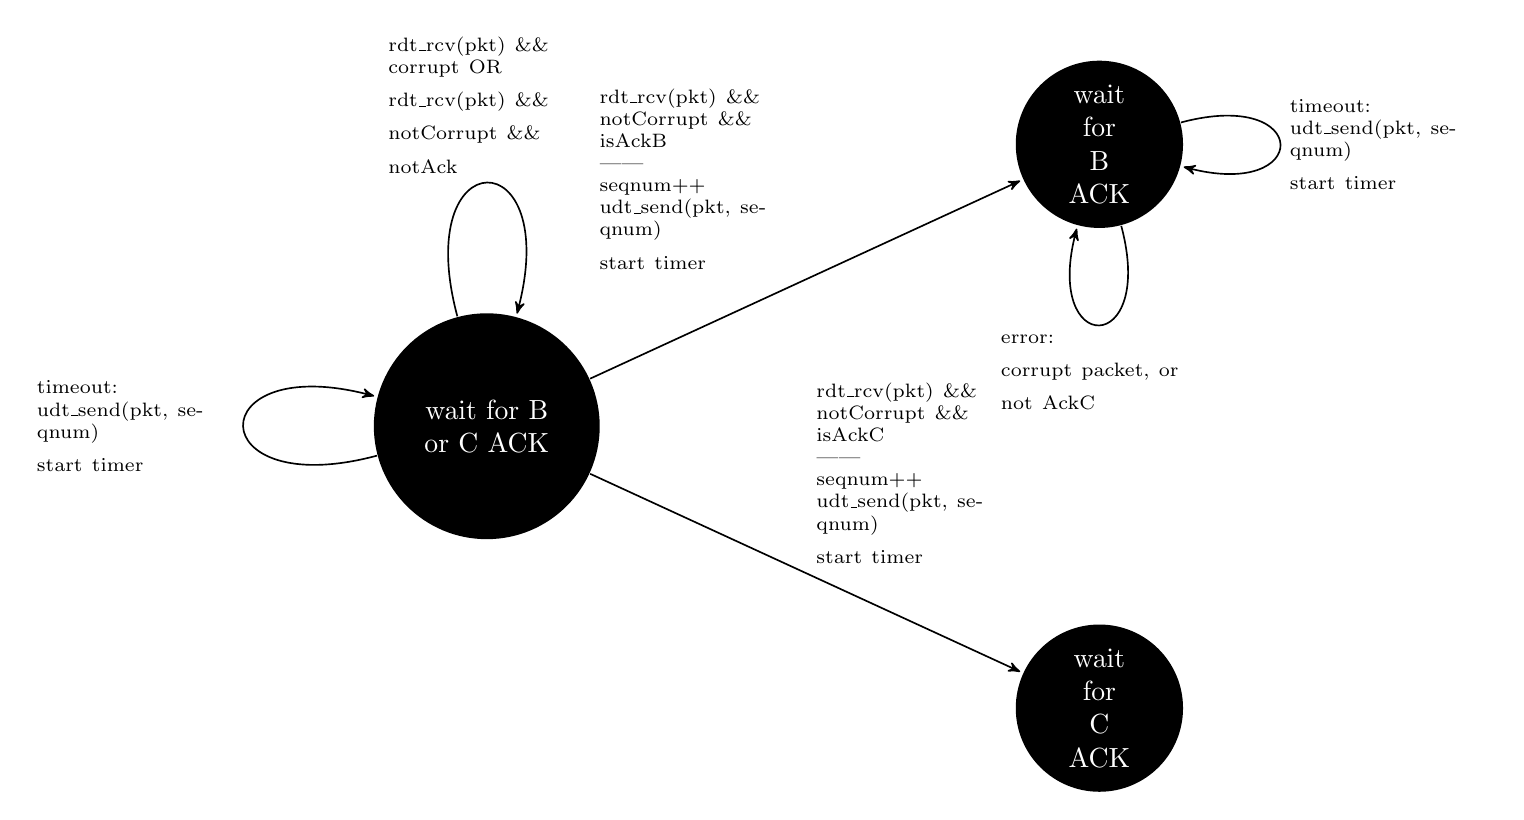
\begin{tikzpicture}[->,>=stealth',shorten >=1pt,auto,node distance=3.8cm,
                    semithick,text width=2.5cm]
  \tikzstyle{every state}=[fill=black,draw=none,text=white,align=center]

  \node[state][text width=2.5cm] (A)  {wait for B or C ACK};
  \node[state][text width=1cm]   (B) [above right=1.8cm and 6cm of A] {wait for\\B ACK};
  \node[state][text width=1cm]   (C) [below right=1.8cm and 6cm of A] {wait for\\C ACK};

  \path (A) edge [loop above] node {\scriptsize rdt\_rcv(pkt) \&\& corrupt OR\\rdt\_rcv(pkt) \&\& notCorrupt \&\& notAck} (A);
  \path (A) edge [loop left] node {\scriptsize timeout:\\udt\_send(pkt, seqnum)\\start timer} (A);
  \path (A) edge node {\scriptsize rdt\_rcv(pkt) \&\& notCorrupt \&\& isAckB\\||\\seqnum++\\udt\_send(pkt, seqnum)\\start timer} (B);
  \path (A) edge node {\scriptsize rdt\_rcv(pkt) \&\& notCorrupt \&\& isAckC\\||\\seqnum++\\udt\_send(pkt, seqnum)\\start timer} (C);
  \path (B) edge [loop right] node {\scriptsize timeout:\\udt\_send(pkt, seqnum)\\start timer} (B);
  \path (B) edge [loop below] node {\scriptsize error:\\corrupt packet, or not AckC} (B);
\end{tikzpicture}

FSM for C:

\item For sender-to-receiver data, the packet format is: seqnum $\vert$ data. For receiver-to-sender control, the packet format is: acknum $\vert$ (B or C).
\item 6d
\end{enumerate}

\item
\begin{enumerate}
\item Consider a server which distributes the data rate of the channel evenly to each peer as $ \frac{u_s}{N} $ bits per second, resulting in the total bandwidth used being $ \frac{u_s}{N} \times N = u_s $. This data rate will not exceed the rate at which clients can receive bits, as it is given that $ \frac{u_s}{N} \leq d_{min} $. If each client is downloading a file of size $ F $ bits, then it will take $ \frac{F}{u_s/N} = \frac{NF}{u_s} $ seconds for each client to download their file.
\item Consider a server which distributes the data rate of the channel to each peer as $ d_{min} $ bits per second, giving a total bandwidth of $ Nd_{min} $. This will not exceed the bandwidth that the server can trasmit, as it is given that $ u_s \geq Nd_{min} $. If each client is downloading a file of size $ F $ bits, then it will take $ \frac{F}{d_min} $ seconds for each client to download their file.
\end{enumerate}

\end{enumerate}
\end{document}
